\section{Materials and Methods}
\subsection{Environment Setup}
To execute this tutorial we will use Python 3.12 \cite{python_download}.

\begin{enumerate}
\item Clone the repository from GitHub:
    \begin{lstlisting}[style=terminal]
    $ git clone https://github.com/JuliaWPereira/fairness
    $ cd fairness
    \end{lstlisting}
\item Create a virtual environment and install the requirements:
    \begin{lstlisting}[style=terminal]
    $ python -m venv .venv
    # Mac / Linux
    $ source .venv/bin/activate

    # Windows CMD:
    $ .venv\Scripts\activate.bat

    # Windows PowerShell:
    $.venv\Scripts\Activate.ps1

    $ pip install "pip <24.1" # to work with fairness
    $ pip install -r requirements.txt
    \end{lstlisting}
\end{enumerate}

We must use pip version lower than 24.1 since Fairness package is malformed at the moment of this tutorial creation (June of $2025$).

We will use \texttt{pandas} package to deal with the dataset of South German credit Data; \texttt{fastparquet} will be used to keep type changes between notebooks, and since parquet is a better structure to datasets; \texttt{numpy} and \texttt{fairness} are used at the numerical exercises; \texttt{matplotlib} and \texttt{seaborn} are used for visualization purposes. \texttt{ydata-profiling} is used to profile the data and analyse correlations and distributions in a faster way; \texttt{ipykernel} is needed to run python notebooks.

\subsection{Dataset}
\subsubsection{Origin and Description}
We employ the South German Credit Data from the UCI Machine Learning Repository \cite{south_2019}, which contains $1000$ anonymized credit applications collected between $1973$ and $1975$. This dataset is a refined version of the classic Statlog German Credit Data \cite{hofmann_statlog_1994}, but fixing some inconsistencies and providing corrections about the background information \cite{south_2019}.

\subsubsection{Feature Types and Preprocessing}

We start analysing the Dataset at the notebook \texttt{notebook/01\_data\_quality.ipynb}.

This dataset contains $14$ categorical variables, $2$ boolean variables, and $3$ numerical variables. Since the columns are written in German, we first translate their names using the codetable provided in \cite{south_2019}. Several features are coded numerically, so we also use the codetable to translate the numbers to interpretable labels.

Please refer to Table \ref{tab:personal} for personal and demographic information, to Table \ref{tab:financial} for financial and employment status, to Table \ref{tab:credit} for credit history and obligations, and to Table \ref{tab:loan} for loan application details.

\begin{table*}[t]
\small
\caption{Personal and Demographic Information}
\begin{tabularx}{\textwidth}{>{\ttfamily}l l X}
\toprule
\label{tab:personal}
\textbf{German Name} & \textbf{English Name} & \textbf{Values / Description} \\
\midrule
alter   & age                     & Applicant's age in years \\
famges  & personal\_status\_sex   & 1: male - divorced/separated; 2: female non-single or male single; 3: male - married/widowed; 4: female - single \\
beruf   & job                     & 1: unemployed/unskilled - non-resident; 2: unskilled - resident; 3: skilled employee/official; 4: manager/self-employed/highly qualified \\
pers    & dependents          & 1: 3 or more; 2: 0 to 2 \\
telef   & telephone               & 1: no; 2: yes (under customer name) \\
gastarb & foreign\_worker         & 1: yes; 2: no \\
\bottomrule
\end{tabularx}
\end{table*}

\begin{table*}[t]
\small
\caption{Financial and Employment Status}
\begin{tabularx}{\textwidth}{>{\ttfamily}l l X}
\toprule
\label{tab:financial}
\textbf{German Name} & \textbf{English Name} & \textbf{Values / Description} \\
\midrule
laufkont  & checking\_account\_status                & 1: no checking account; 2: balance < 0 DM; 3: 0–200 DM; 4: ≥200 DM or salary ≥1 year \\
sparkont  & savings\_account\_balance               & 1: no/unknown; 2: < 100 DM; 3: 100–499 DM; 4: 500–999 DM; 5: ≥ 1000 DM \\
beszeit   & employment\_duration  & 1: unemployed; 2: < 1 yr; 3: 1–4 yrs; 4: 4–7 yrs; 5: ≥ 7 yrs \\
verm      & property              & 1: no property; 2: car or other; 3: life insurance/savings; 4: real estate \\
rate      & installment\_rate     & 1: ≥35\%; 2: 25–34\%; 3: 20–24\%; 4: <20\% \\
wohn      & housing               & 1: for free; 2: rent; 3: own \\
wohnzeit  & residence\_since    & 1: <1 yr; 2: 1–3 yrs; 3: 4–6 yrs; 4: ≥7 yrs \\
\bottomrule
\end{tabularx}
\end{table*}

\begin{table*}[t]
\small
\caption{Credit History and Obligations}
\begin{tabularx}{\textwidth}{>{\ttfamily}l l X}
\toprule
\label{tab:credit}
\textbf{German Name} & \textbf{English Name} & \textbf{Values / Description} \\
\midrule
moral     & credit\_history           & 0: delayed repayment; 1: critical account; 2: no credits or all paid; 3: current credits paid; 4: all bank credits paid \\
buerge    & guarantors            & 1: none; 2: co-applicant; 3: guarantor \\
bishkred  & existing\_credits\_count           & 1: 1; 2: 2–3; 3: 4–5; 4: ≥6 \\
weitkred  & other\_installment\_plans & 1: bank; 2: stores; 3: none \\
\bottomrule
\end{tabularx}
\end{table*}

\begin{table*}[t]
\small
\caption{Loan Application Details}
\begin{tabularx}{\textwidth}{>{\ttfamily}l l X}
\toprule
\label{tab:loan}
\textbf{German Name} & \textbf{English Name} & \textbf{Values / Description} \\
\midrule
laufzeit & duration\_months         & Duration of requested loan (in months) \\
hoehe    & credit\_amount           & Requested loan amount (in Deutsche Marks) \\
verw     & purpose          & 0: others; 1: car (new); 2: car (used); 3: furniture; 4: TV/radio; 5: appliances; 6: repairs; 7: education; 8: vacation; 9: retraining; 10: business \\
kredit   & credit\_risk      & 0: bad credit; 1: good credit \\
\bottomrule
\end{tabularx}
\end{table*}

\subsubsection{Target Variable}
The binary target variable, \texttt{credit\_risk}, represents the bank's assessment of the applicant: \texttt{0 = bad credit} and \texttt{1 = good credit}. It is important to note that the dataset contains an oversampled number of bad credit cases—a common approach in domains with imbalanced outcomes. However, this means that the observed class distribution does not reflect the real-world prevalence of defaults, showed in Fig. \ref{fig:creditdist}.

\begin{figure}[ht]
\centering
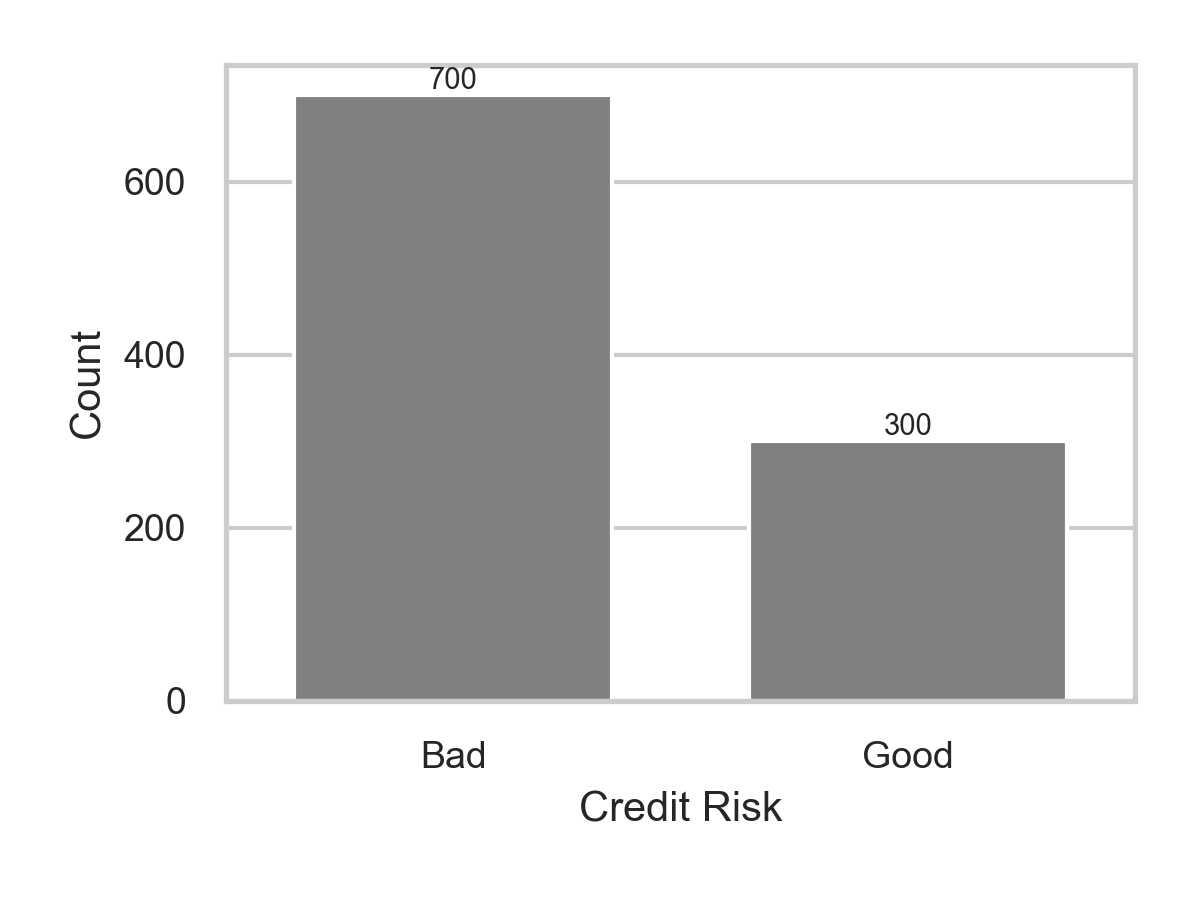
\includegraphics[width=0.9\linewidth]{figures/credit_risk_distribution.png}
\caption{Credit risk distribution (good vs bad).}
\label{fig:creditdist}
\end{figure}

\subsubsection{Sensitive Attributes and Proxy Risk}
We identify three features as sensitive for the purposes of fairness analysis:
\begin{itemize}
    \item \textbf{age} -- a continuous variable that may be subject to age-based discrimination;
    \item \textbf{foreign\_worker} -- a binary variable associated with nationality and potential racial bias;
    \item \textbf{personal\_status\_sex} -- a categorical feature encoding both gender and marital status.
\end{itemize}

In addition to directly sensitive attributes, we must also consider \textit{proxy attributes}: variables that are not explicitly sensitive but may carry correlated information about protected characteristics~\cite{pessach2020algorithmic}. For example, employment duration or housing status may reveal age-related patterns, while credit amount may indirectly relate to gender roles in financial responsibility. In Subsection~\ref{subsubsec:sensitive}, we present an empirical analysis of such correlations to identify latent proxies.

\section{Tutorial Workflow}

In this section, we outline the full pipeline used to audit and mitigate bias in the South German Credit dataset. The process is divided into seven distinct stages, each aimed at identifying, quantifying, and addressing potential algorithmic unfairness. 

\subsection{Pipeline Overview}
The tutorial follows this sequence:
\begin{enumerate}
    \item Data loading and initial preprocessing (already explained at the setup process);
    \item Mapping sensitive and proxy attributes;
    \item Exploratory Data Analysis (EDA): feature distribution, class balance, and sensitive attribute correlation;
    \item Base model training: Logistic Regression and Decision Trees using Scikit-learn;
    \item Fairness Evaluation: applying metrics such as Demographic Parity Difference and Equal Opportunity Difference using AIF360;
    \item Bias Mitigation: using pre-processing (Reweighing) and post-processing (Reject Option Classification) techniques;
    \item Result Comparison: measuring accuracy and fairness before and after mitigation.
\end{enumerate}

Each step is detailed in the following subsections.


% \subsubsection{Mapping Sensitive and Proxy Attributes}\label{subsubsec:sensitive}
% Three sensitive variables were selected: \texttt{age}, \texttt{foreign\_worker}, and \texttt{personal\_status\_sex}. We also analyzed potential proxy variables using correlation and mutual information to determine whether non-sensitive features encode sensitive information indirectly.

% To support this analysis, we computed and visualized the top features most strongly correlated or informationally linked to each sensitive variable. These visualizations help identify potential proxy attributes that may leak sensitive information.

% In Fig. \ref{fig:proxy_age} the most correlated features with \texttt{age} are \texttt{employment\_duration}, \texttt{residence\_since}, and \texttt{job}, which are clearly related to one person's stage in life. This is an indicator that those features may be proxy sensitive, indicating a risk of age-related patterns within them.

% \begin{figure}[!ht]
% \centering
% 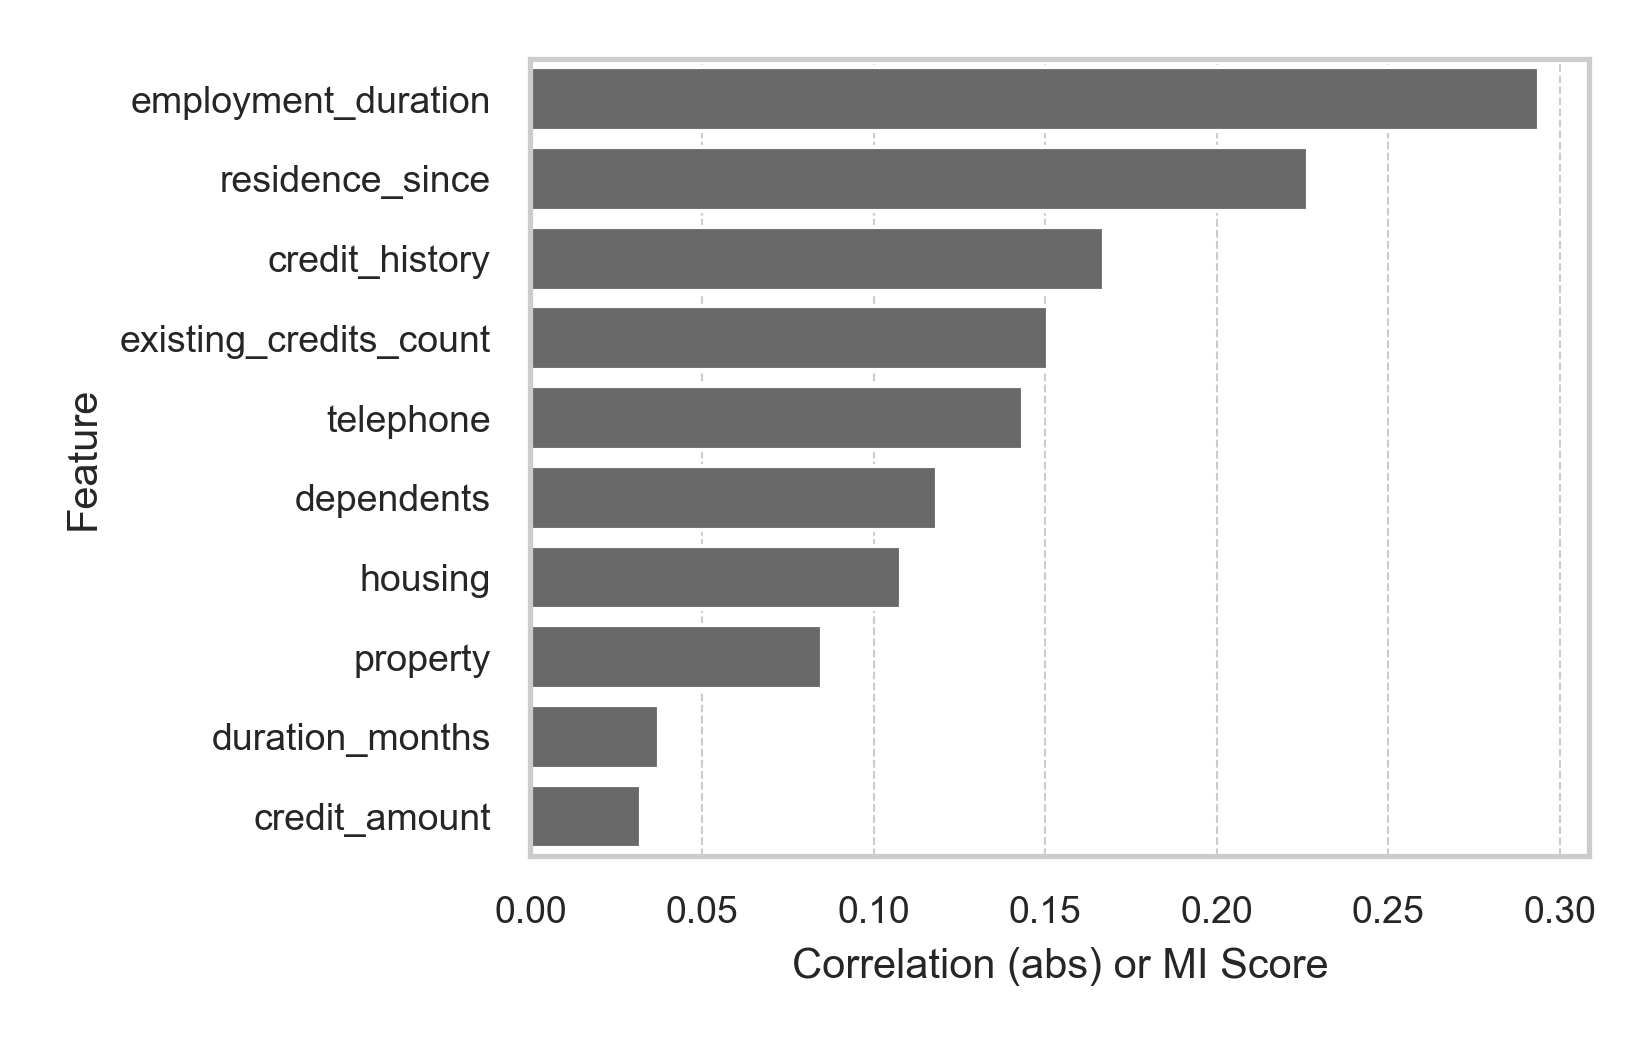
\includegraphics[width=0.85\linewidth]{figures/age_proxy_plot.png}
% \caption{Top correlated and informative features with \texttt{age}.}
% \label{fig:proxy_age}
% \end{figure}

% In Fig. \ref{fig:proxy_foreign}, there is a moderate information gain from \texttt{credit\_amount}, which indicates that financial variables such as previous credit provided may reflect differences in treatment for foreign applicants.

% \begin{figure}[!ht]
% \centering
% 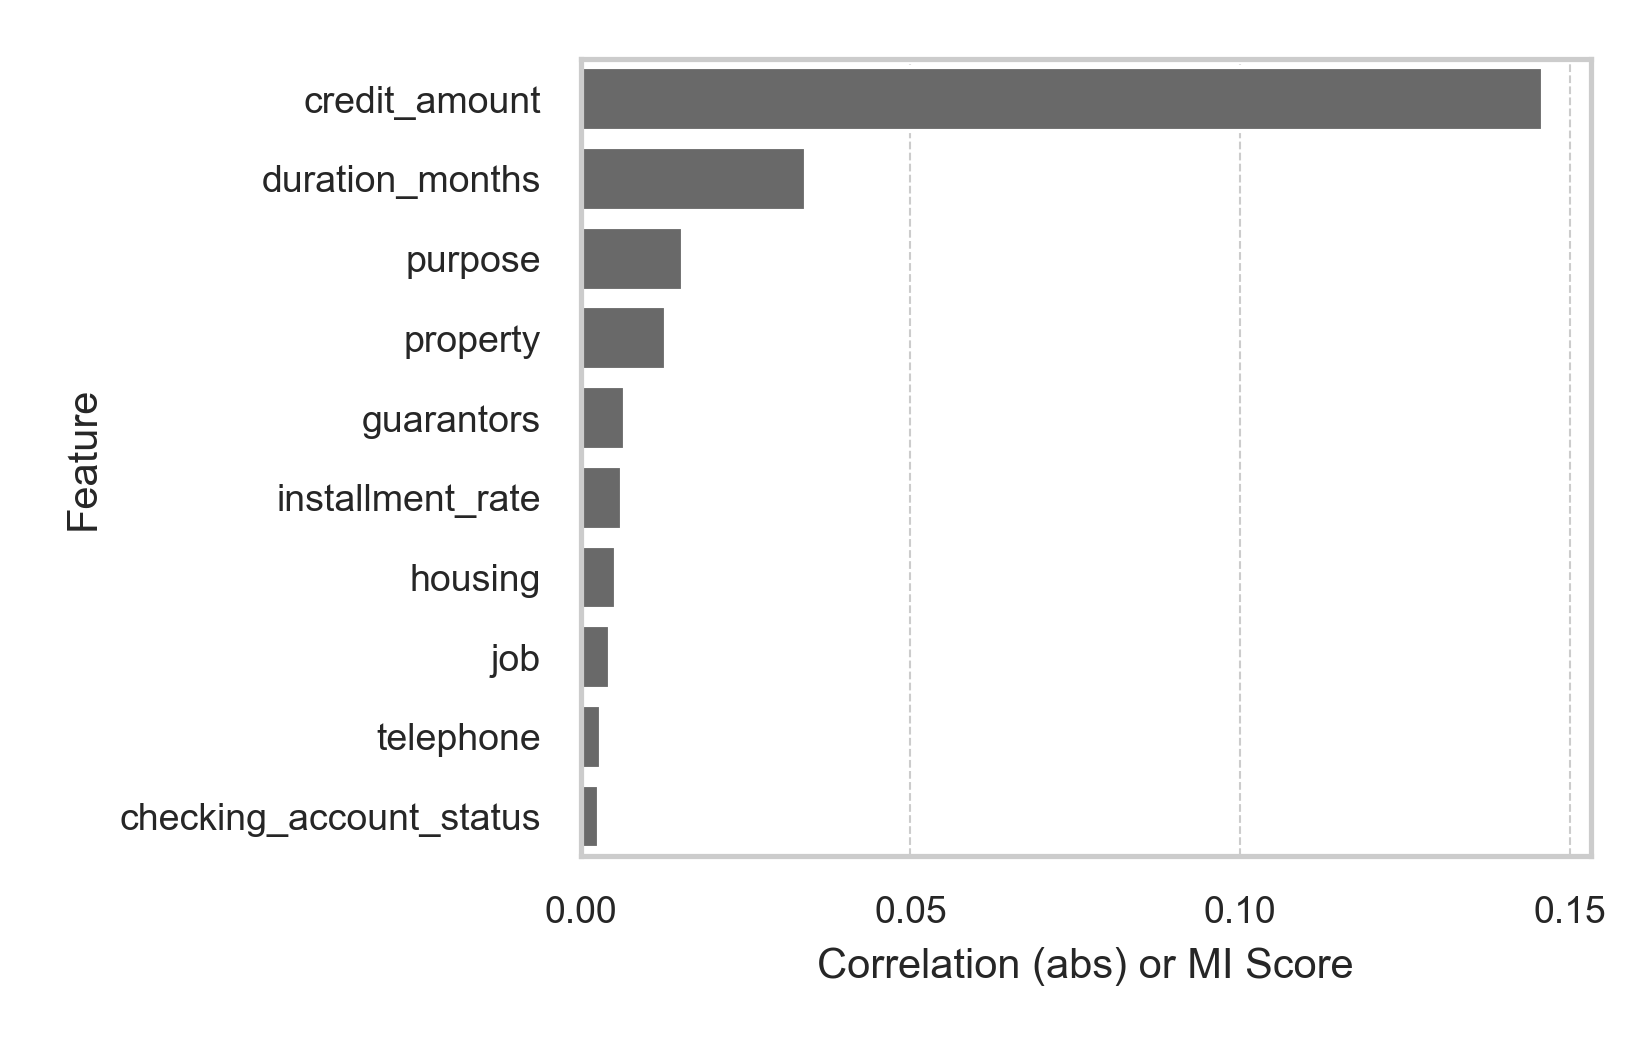
\includegraphics[width=0.85\linewidth]{figures/foreign_worker_proxy_plot.png}
% \caption{Top correlated and informative features with \texttt{foreign\_worker}.}
% \label{fig:proxy_foreign}
% \end{figure}

% In Fig. \ref{fig:proxy_sex}, there is a considerable high correlation between \texttt{personal\_status\_sex} and \texttt{credit\_amount}, which indicates again that this financial variable may bring unfairness to the model. For now we will include \texttt{credit\_amount} as a \textbf{sensitive proxy attribute}.

% \begin{figure}[!ht]
% \centering
% 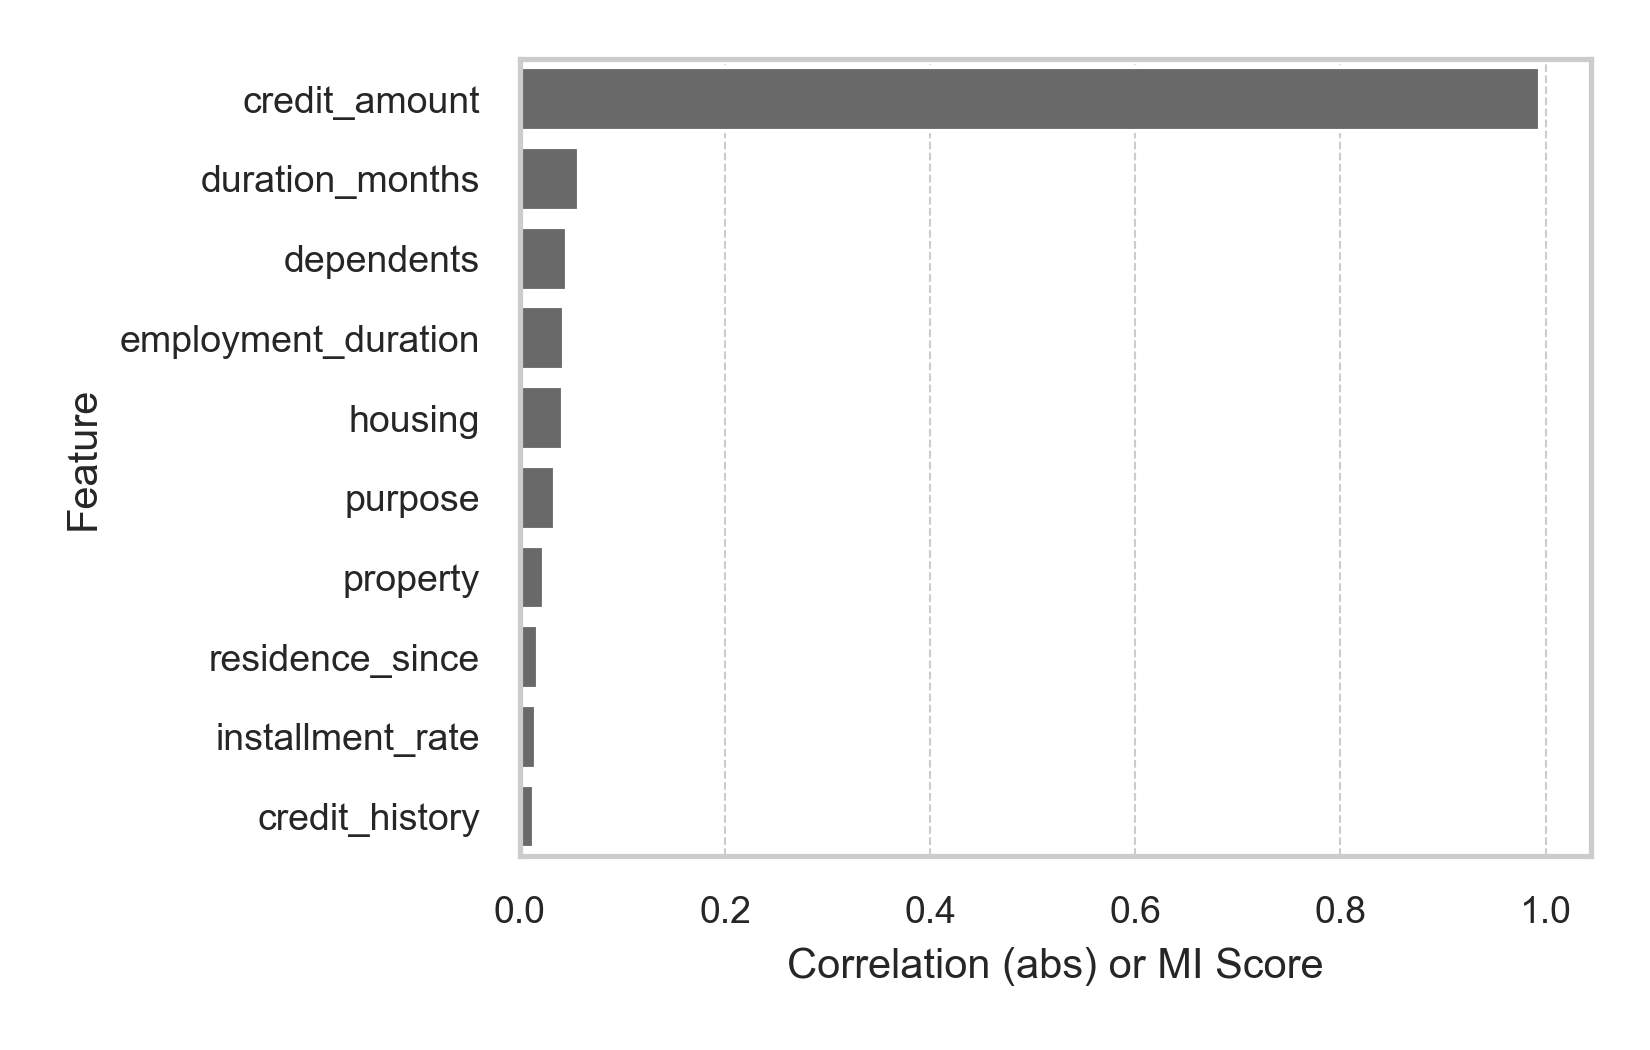
\includegraphics[width=0.85\linewidth]{figures/personal_status_sex_proxy_plot.png}
% \caption{Top correlated and informative features with \texttt{personal\_status\_sex}.}
% \label{fig:proxy_sex}
% \end{figure}

\subsection{Mapping Sensitive and Proxy Attributes}

We define the following features as \textbf{sensitive attributes} for fairness evaluation:

\begin{itemize}
    \item \texttt{age} – a continuous variable potentially subject to age-based discrimination;
    \item \texttt{foreign\_worker} – a binary variable associated with nationality;
    \item \texttt{personal\_status\_sex} – a categorical feature combining gender and marital status.
\end{itemize}

To identify \textbf{proxy attributes}, we use two statistical approaches: \textit{Pearson correlation}, to capture linear relationships, and \textit{mutual information} (MI), to detect nonlinear dependencies. Since some features are categorical, we first encode them numerically.

\begin{lstlisting}[language=Python, caption=Encoding categorical features, frame=single]
from sklearn.preprocessing import LabelEncoder

df_encoded = df.copy()
for col in df_encoded.select_dtypes(include='object'):
    df_encoded[col] = LabelEncoder().fit_transform(df_encoded[col])
\end{lstlisting}

We then assess which features leak information about \texttt{age} by computing correlations and mutual information with a binned version of age:

\begin{lstlisting}[language=Python, caption=Analyzing proxy risk for age, frame=single]
df_encoded['age_group'] = pd.qcut(df['age'], q=4, labels=False)

from sklearn.feature_selection import mutual_info_classif

X = df_encoded.drop(columns=['age', 'age_group'])
y = df_encoded['age_group']
mi = mutual_info_classif(X, y)
\end{lstlisting}

At Table \ref{tab:mi_thresholds} we establish thresholds to understand which variables are really at risk to be proxy or just potential ones.

\begin{table}[h]
\centering
\caption{Qualitative guidelines for interpreting Mutual Information (MI) scores in proxy detection.}
\label{tab:mi_thresholds}
\begin{tabular}{lc}
\toprule
\textbf{MI Score Range} & \textbf{Interpretation} \\
\midrule
0.00 -- 0.02   & Very weak / no dependency \\
0.02 -- 0.07   & Weak dependency (likely safe) \\
0.07 -- 0.15   & Moderate proxy potential \\
$>$ 0.15       & Strong proxy risk (flag feature) \\
\bottomrule
\end{tabular}

\vspace{0.5em}
\small
\textit{Note:} These thresholds are based on guidelines from feature selection heuristics~\cite{peng2005feature}, mutual information-based filtering for fairness~\cite{calmon2017optimized}, and practical usage in AIF360~\cite{bellamy2019aif360}.
\end{table}

\begin{table*}[ht]
\small
\centering
\caption{Features identified as likely or potential proxies for sensitive attributes based on mutual information. Likely proxies (MI $>$ 0.15 for at least one attribute) are listed first and shown in \textbf{bold}.}
\label{tab:sorted_mi_proxies}
\begin{tabular}{lrrr>{\itshape}c}
\toprule
\textbf{Feature} & \textbf{Age} & \textbf{Foreign Worker} & \textbf{Personal Status / Sex} & \textbf{Proxy Status} \\
\midrule
\textbf{employment\_duration}     & \textbf{0.294} &         & 0.063 & likely\_proxy \\
\textbf{residence\_since}         & \textbf{0.227} & 0.045   &       & likely\_proxy \\
\textbf{credit\_history}          & \textbf{0.167} & 0.039   & 0.102 & likely\_proxy \\
\textbf{existing\_credits\_count} & \textbf{0.151} &         & 0.114 & likely\_proxy \\
\textbf{dependents}               & 0.119          & 0.077   & \textbf{0.267} & likely\_proxy \\
\textbf{housing}                  & 0.108          & 0.033   & \textbf{0.184} & likely\_proxy \\
credit\_amount                    & 0.032          &         & 0.149 & potential\_proxy \\
guarantors                        &                & 0.120   &       & potential\_proxy \\
duration\_months                  & 0.038          & 0.135   & 0.118 & potential\_proxy \\
telephone                         & 0.144          & 0.075   & 0.087 & potential\_proxy \\
\bottomrule
\end{tabular}
\end{table*}



The top correlated and informative features for \texttt{age} are shown in Figure~\ref{fig:proxy_age}. We observe that variables such as \texttt{employment\_duration}, \texttt{residence\_since}, and \texttt{credit\_history} and \texttt{existing\_credits\_count}. This makes sense since older applicants tend to have longer employment history, longer time at a residence and more stable credit histories.

\begin{figure}[ht]
\centering
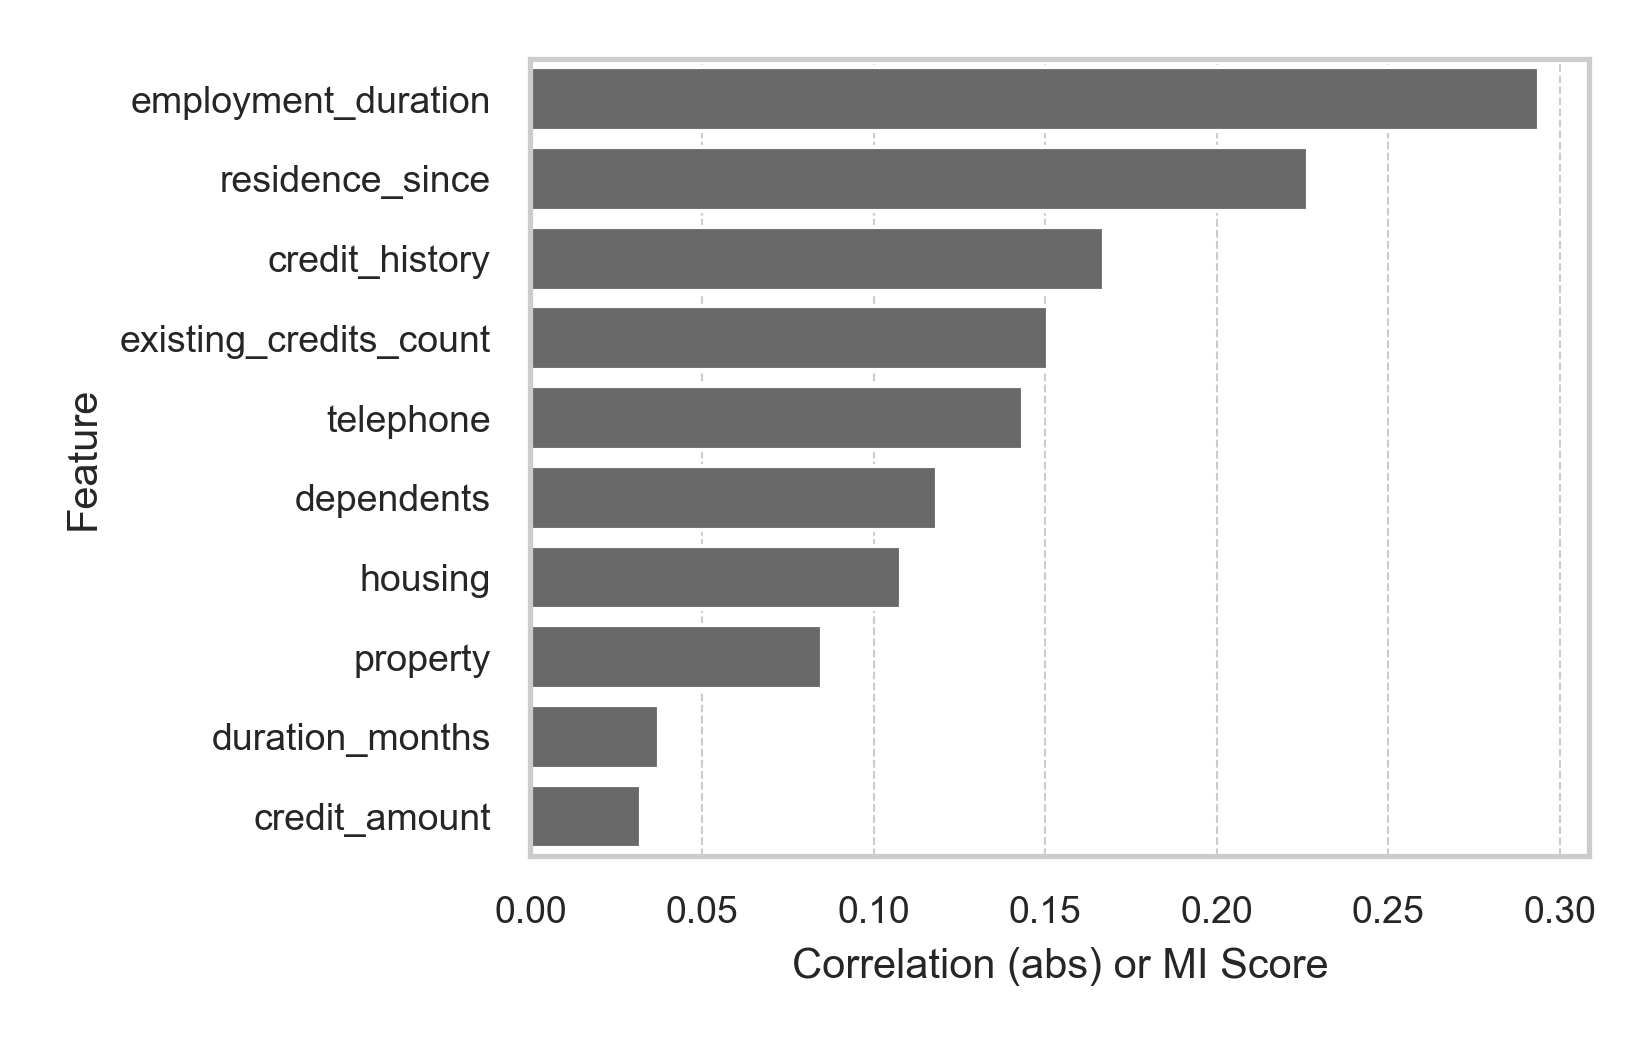
\includegraphics[width=\linewidth]{figures/age_proxy_plot.png}
\caption{Top correlated and informative features with \texttt{age}.}
\label{fig:proxy_age}
\end{figure}

We repeat this process for \texttt{foreign\_worker} and \texttt{personal\_status\_sex}, using the original categorical labels as targets. 

For \texttt{foreign\_worker}, there is no strong alert to a proxy, we have only two potential proxies with \texttt{duration\_months} and \texttt{guarantors}, what makes sense with a more conservative approach in cases with foreigners which does not have a large credit history in the country to ask for guarantors.

In both cases, features such as \texttt{credit\_amount}, \texttt{housing}, and \texttt{employment\_duration} show high MI values, revealing indirect bias risks.

\begin{figure}[ht]
\centering
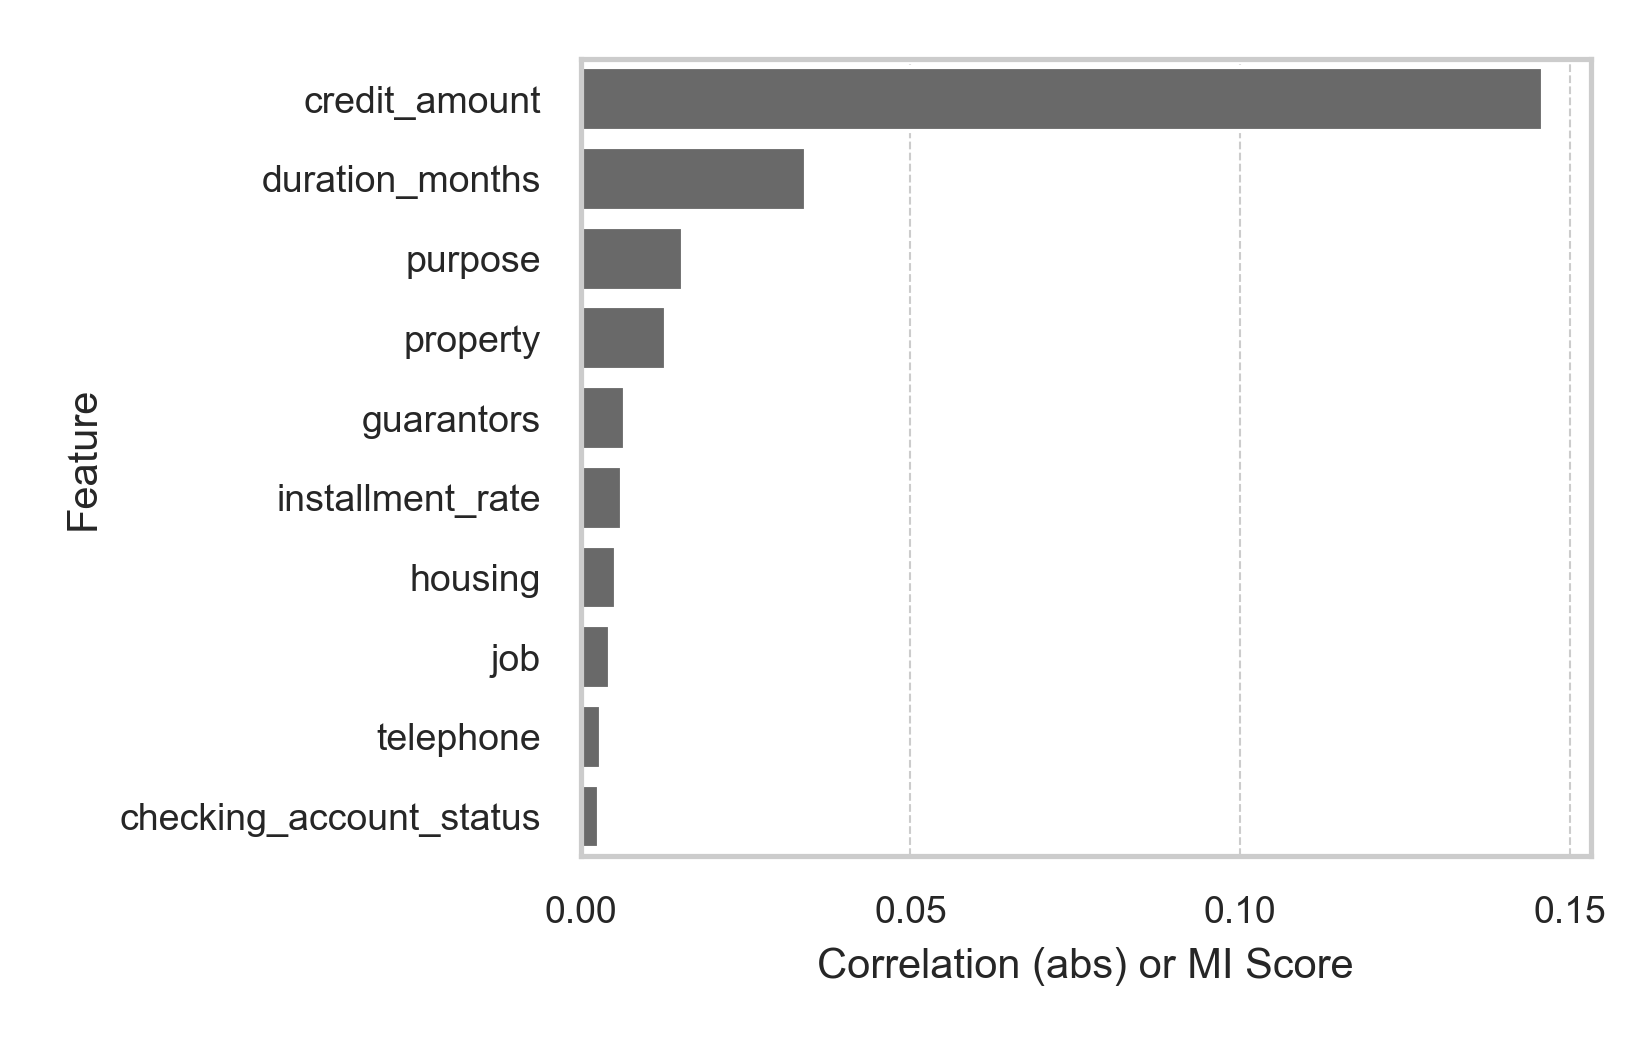
\includegraphics[width=\linewidth]{figures/foreign_worker_proxy_plot.png}
\caption{Top features linked to \texttt{foreign\_worker} status.}
\label{fig:proxy_foreign_worker}
\end{figure}

\begin{figure}[ht]
\centering
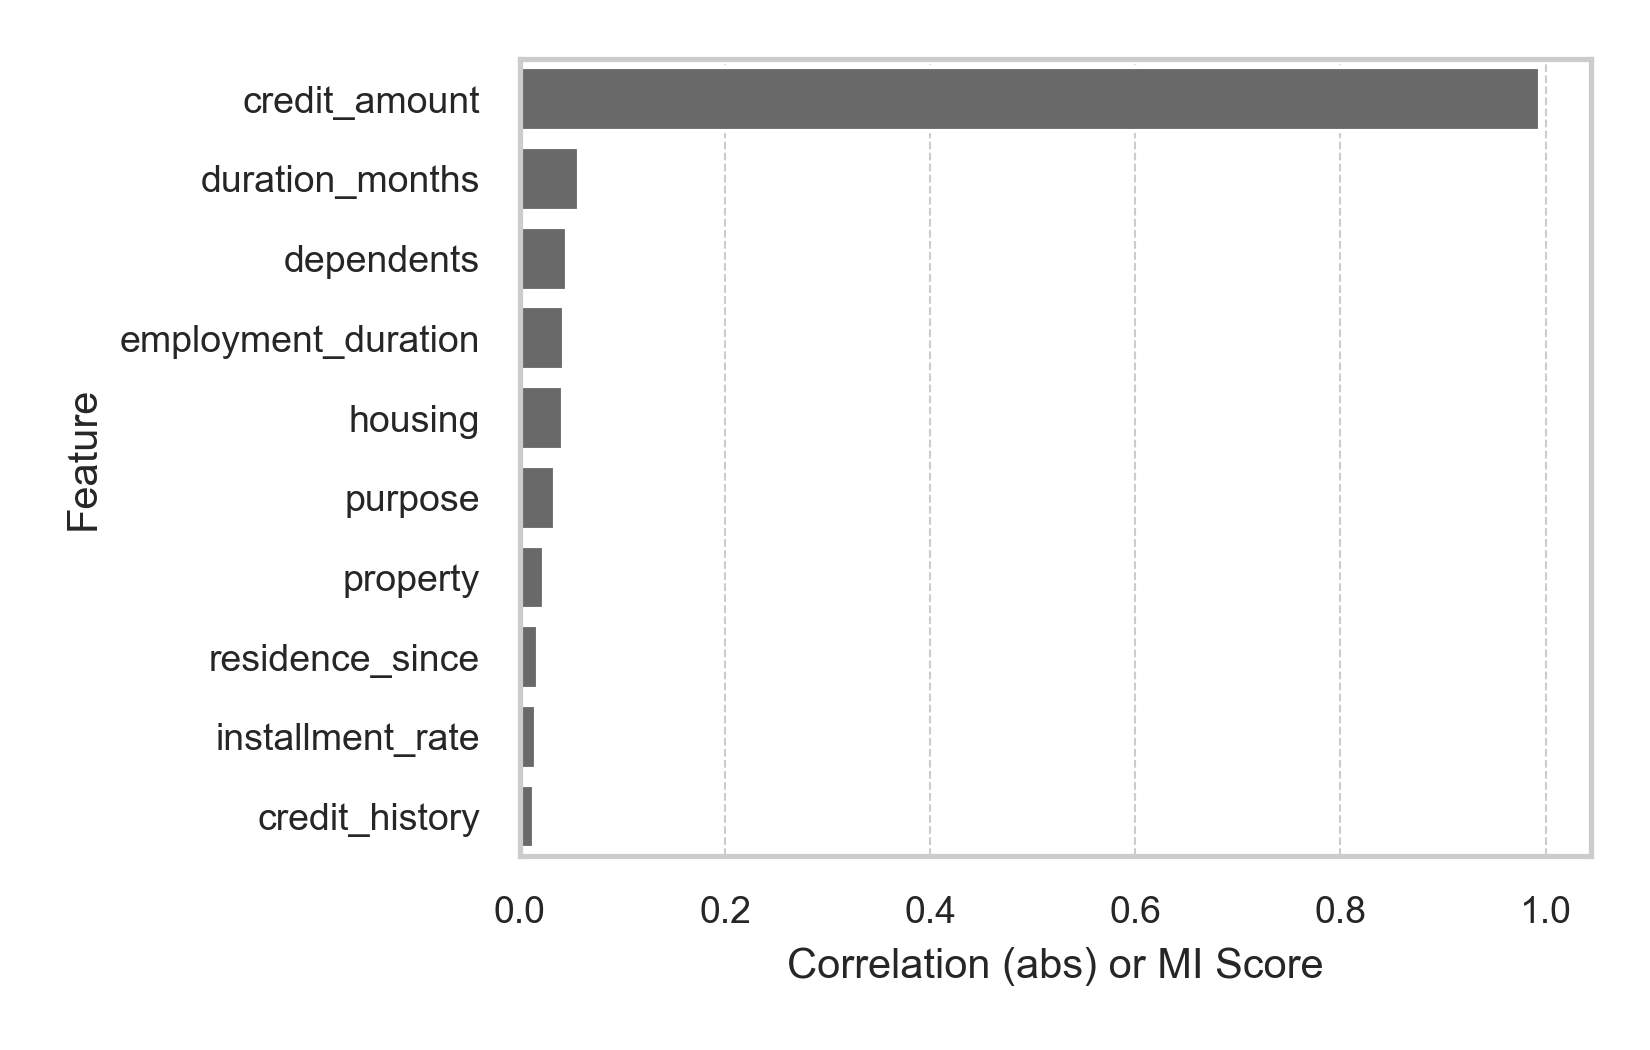
\includegraphics[width=\linewidth]{figures/personal_status_sex_proxy_plot.png}
\caption{Top features associated with \texttt{personal\_status\_sex}.}
\label{fig:proxy_status_sex}
\end{figure}

These results justify the need to monitor not only sensitive attributes but also proxy features that may introduce bias unintentionally. In our mitigation strategy, we either account for or explicitly adjust these correlations to improve fairness outcomes.


\subsubsection{Exploratory Data Analysis (EDA)}
We examined the distribution of each feature, checked for class balance, and visualized relationships between the target and sensitive attributes.

In Fig. \ref{fig:age_vs_credit_risk} we can notice that the applicants with bad credit tend to be slightly younger on average in comparison with good credit risk ones. The bad curve also has a earlier around late 20s, while the good group is more spreaded. It suggests that age plays an implicit role in credit evaluation.

\begin{figure}[!ht]
\centering
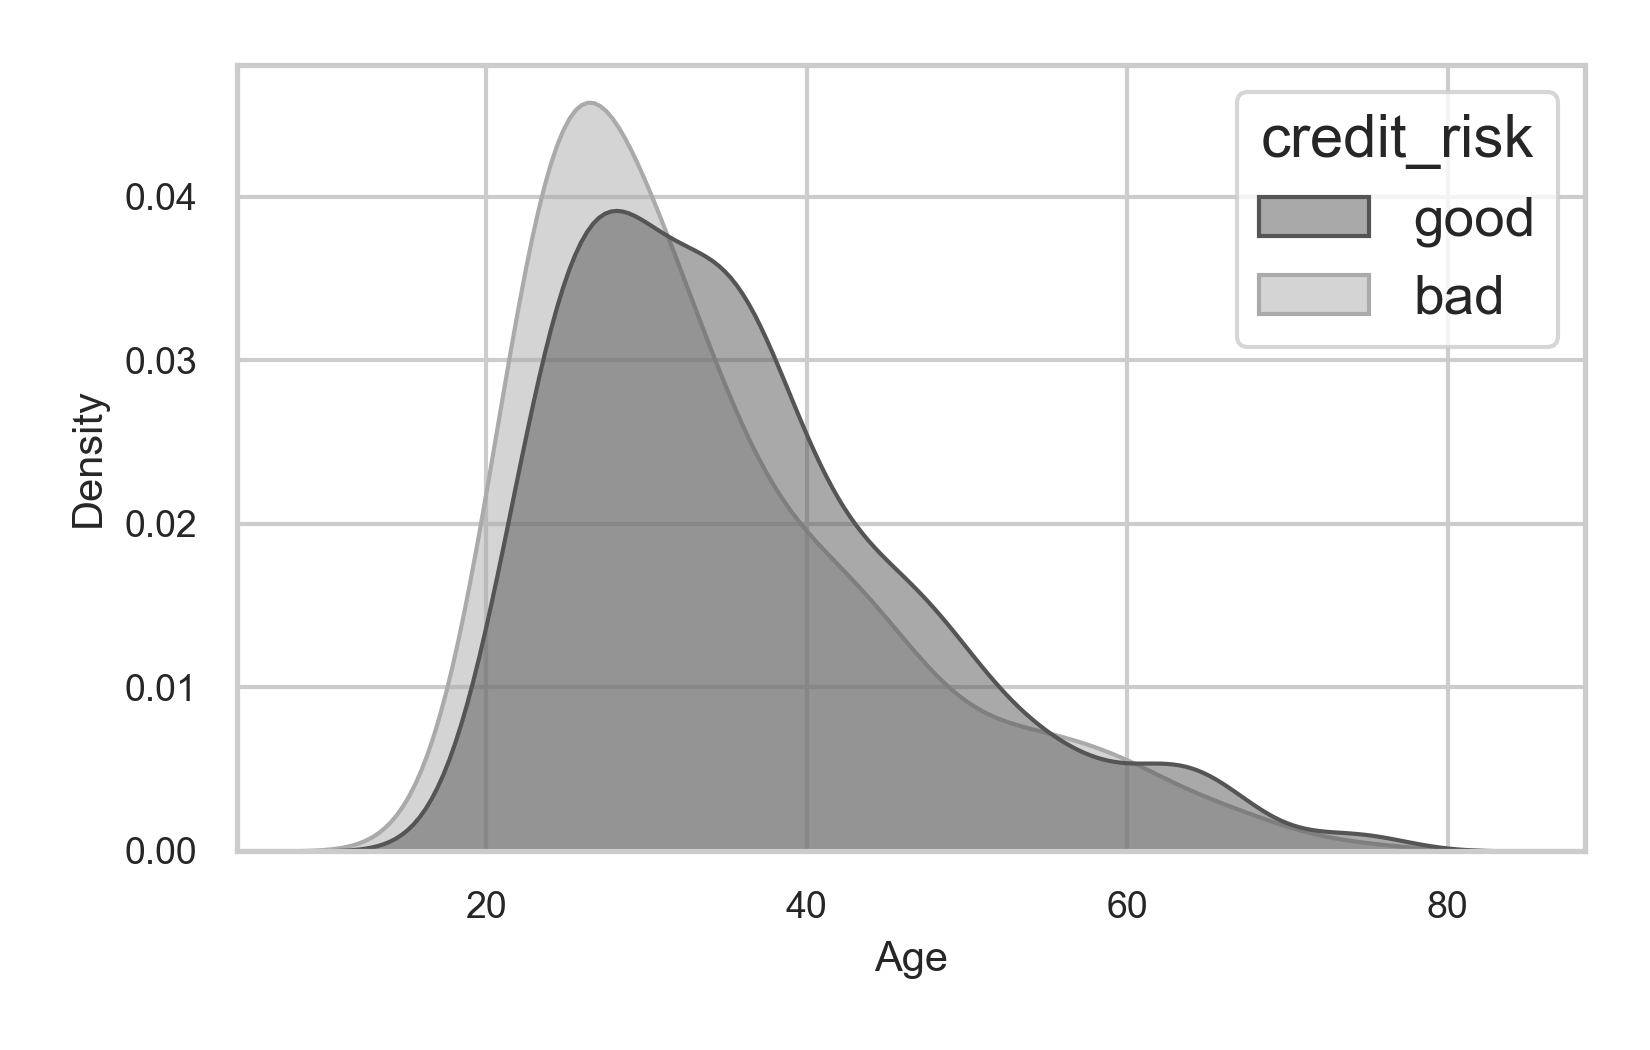
\includegraphics[width=0.85\linewidth]{figures/age_distribution_by_credit_risk.png}
\caption{Age vs. Credit Risk.}
\label{fig:age_vs_credit_risk}
\end{figure}

In Fig. \ref{fig:foreigner_vs_credit_risk} we can notice that the disparity between domestic applicants (\texttt{Foreign Worker == 'no'}) receiving \textbf{good} credit rating is high ($667$ good compared to $296$ bad credit rating) while for foreigners it is considerably lower ($33$ good compared to $4$ bad credit). Notice also that the foreigner group is under-represented (only $3.7\%$ of the total data), limiting the model's ability to generalize fairly for this group, what amplifies the risk of discrimination.

\begin{figure}[!ht]
\centering
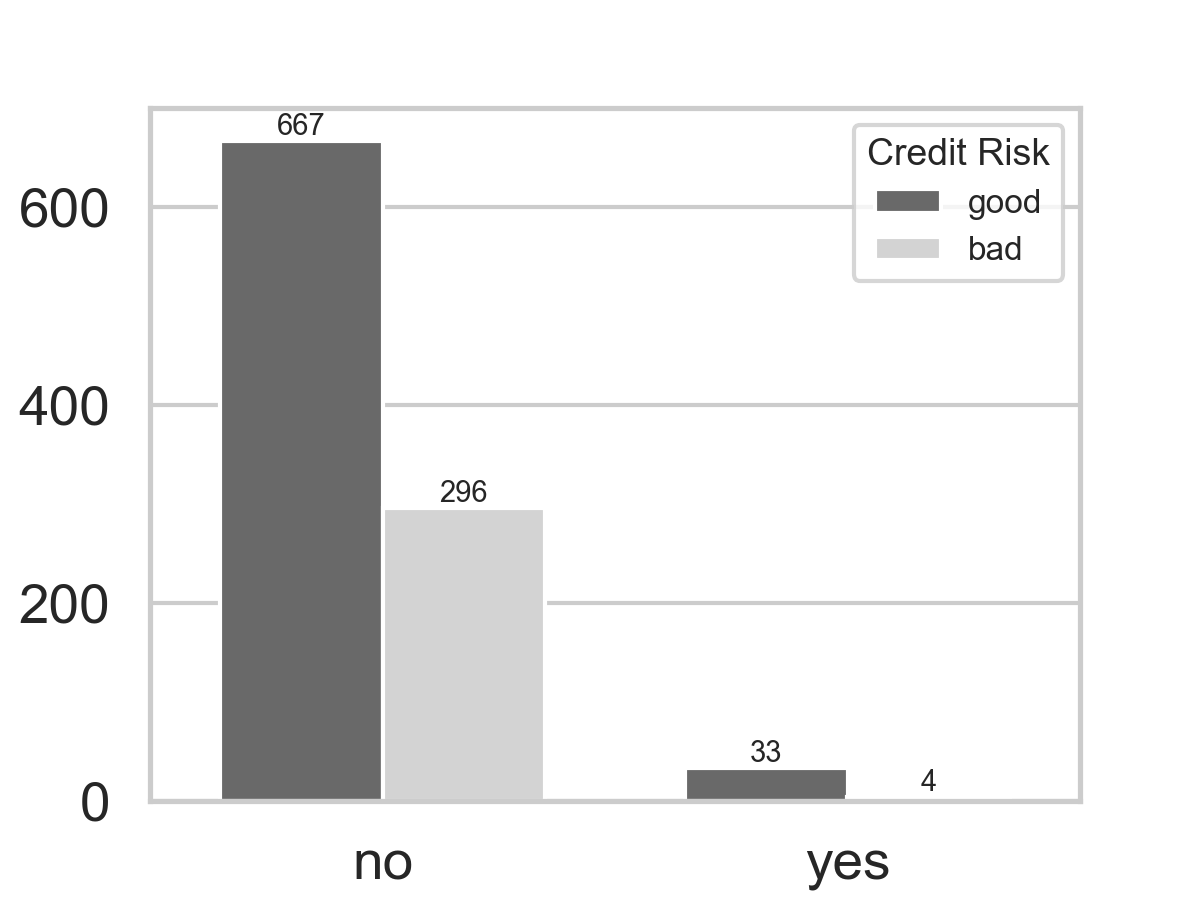
\includegraphics[width=0.85\linewidth]{figures/foreign_worker_vs_credit_risk.png}
\caption{Foreigner Worker vs. Credit Risk.}
\label{fig:foreigner_vs_credit_risk}
\end{figure}

For gender-status subgroups there are substantial differences. Male applicants, if married or widowed, receive the major number of approvals, followed by female applicants which are non-single or single male. In contrast, single female and divorced male have lower absolute counts and more balanced negative distribution. These differences suggest that marital status and gender may influence credit decisions. The underlying historical bias in these categories may result in unfair treatment, especially for under-represented groups such as single women or divorced men.

\begin{figure}[!ht]
\centering
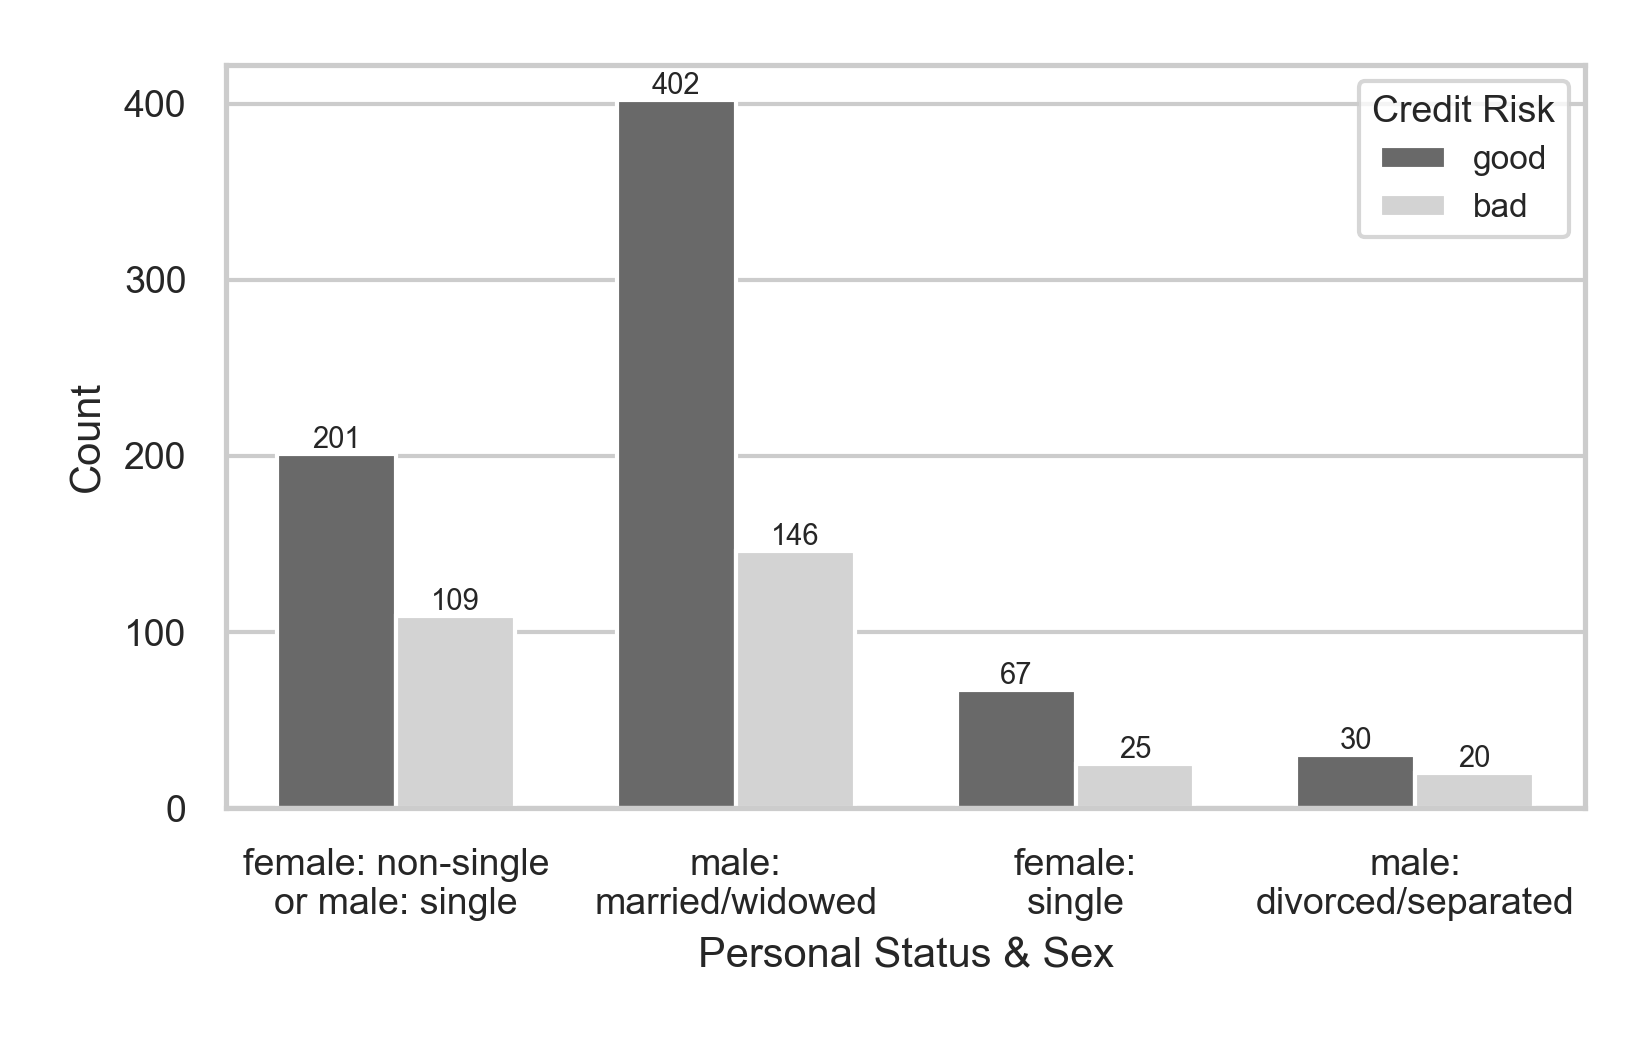
\includegraphics[width=0.85\linewidth]{figures/credit_risk_personal_status_final.png}
\caption{Personal Status vs. Credit Risk.}
\label{fig:personal_status_vs_credit_risk}
\end{figure}

\subsubsection{Baseline Model: Random Forest}

Following the Statlog benchmark, we implemented a Random Forest classifier using Scikit-learn with 100 estimators and default hyperparameters. The dataset was split into training and test sets with a 70/30 ratio, and one-hot encoding was applied to categorical features. The sensitive attributes were excluded from training to simulate fairness through unawareness.

The model achieved an overall accuracy of 0.76. The classification report showed higher recall and precision for the positive class (good credit), but poor performance in identifying bad credit cases:

\begin{itemize}
    \item \textbf{Accuracy:} 0.76
    \item \textbf{F1-score (class 0):} 0.48
    \item \textbf{F1-score (class 1):} 0.84
\end{itemize}

\subsubsection{Fairness Evaluation}
To evaluate fairness, we computed the \textit{Demographic Parity Difference (DPD)} across three sensitive attributes: \texttt{foreign\_worker}, \texttt{personal\_status\_sex}, and binned \texttt{age}. The results revealed the following disparities in selection rates between groups:

\begin{itemize}
    \item \textbf{DPD (foreign\_worker):} 0.2517
    \item \textbf{DPD (personal\_status\_sex):} 0.1512
    \item \textbf{DPD (age):} 0.0580
\end{itemize}

These disparities indicate that the model indirectly encodes bias through correlated features, even when sensitive variables are excluded. This motivates the need for mitigation techniques in the next stage.
\subsubsection{Fairness Mitigation via Reweighing}

To mitigate group-based disparities, we applied the Reweighing algorithm from the AIF360 toolkit~\cite{aif360}. This pre-processing method adjusts the instance weights to reduce bias in the training data, without altering the features or labels. We defined \texttt{foreign\_worker} as the protected attribute, with “yes” as the privileged group.

We trained a Random Forest classifier on the reweighted dataset using the same architecture as before. The model achieved a higher overall accuracy of \textbf{0.839}, while significantly reducing the demographic disparity observed prior to mitigation.

\begin{itemize}
    \item \textbf{Accuracy after reweighing:} 0.839
    \item \textbf{DPD after reweighing:} 0.0705
\end{itemize}

Compared to the baseline model (DPD = 0.2517), this result demonstrates that reweighing is effective in reducing bias while preserving or even improving predictive performance.


\subsubsection{Result Comparison}
Table~\ref{tab:comparison} summarizes the performance and fairness trade-offs between the baseline model and the mitigated model using reweighing. While the reweighted model improved overall accuracy, it also significantly reduced demographic disparities across all evaluated attributes.

\begin{table}[h]
\centering
\caption{Comparison of Accuracy and Fairness Before and After Reweighing}
\label{tab:comparison}
\begin{tabular}{lccc}
\toprule
\textbf{Model} & \textbf{Accuracy} & \textbf{DPD (FW / PS / Age)} \\
\midrule
Baseline RF & 0.753 & 0.2517 / 0.1512 / 0.0580 \\
Reweighed RF & 0.839 & 0.0705 / 0.0814 / 0.0453 \\
\bottomrule
\end{tabular}
\end{table}

These results demonstrate that fairness-aware preprocessing can reduce bias across multiple dimensions while maintaining or even improving predictive performance.





